\documentclass[letterpaper,11pt]{article}
\usepackage[spanish]{babel}
\usepackage[utf8]{inputenc}
\usepackage[T1]{fontenc}
\usepackage{graphicx}
\usepackage{geometry}
\usepackage{array,longtable,booktabs}
\usepackage{setspace}
\usepackage{titlesec}
\usepackage[shortlabels]{enumitem}
\usepackage{amsmath,amssymb,amsfonts,amsthm}
\usepackage{float}
\usepackage{xcolor}
\usepackage{realboxes}
\usepackage{fancyhdr}
\usepackage{anysize}
\usepackage{hyperref}
\usepackage{verbatim}
\usepackage{icomma}
\usepackage{tikz}
\usepackage{pgfplots}
\usepackage{framed}
\usetikzlibrary{arrows,decorations.fractals,decorations.pathmorphing,shadows}
\pgfplotsset{compat=1.18}
\geometry{margin=2.5cm}
\definecolor{lightgrey}{rgb}{0.95,0.95,0.95}
\newcommand{\code}[1]{\Colorbox{lightgrey}{\texttt{#1}}}
\newcommand{\s}{\vspace{0.2cm}}
\newcommand{\R}{{\mathbb R}}
\newcommand{\C}{{\mathbb C}}
\newcommand{\Z}{\mathbb{Z}}
\newcommand{\N}{{\mathbb N}}
\newcommand{\ds}{\displaystyle}
\newcommand{\sen}{\mathop{\rm sen}\nolimits}
\newcommand{\n}{\noindent}
\newcommand{\ex}{\mathop{\rm e}\nolimits}
\newcommand{\ssi}{\Longleftrightarrow}
\newcommand{\implica}{\Longrightarrow}
\DeclareMathOperator{\var}{Var}
\DeclareMathOperator{\cov}{Cov}
\DeclareMathOperator{\Exp}{\mathbb{E}}
\newcommand{\E}[1]{\Exp\left[#1\right]}
\DeclareMathOperator{\plim}{plim}
\DeclareMathOperator{\Prob}{\mathbb{P}}
\newcommand{\prob}[1]{\Prob\left(#1\right)}
\newcommand{\abs}[1]{\left|#1\right|}
\newcommand{\pto}{\xrightarrow{p}}
\newcommand{\respuesta}{\color{blue}\paragraph{Respuesta.}}
\newcommand{\fin}{\color{black}}
\pagestyle{fancy}
\fancyhf{}
\fancyhead[L]{INGENIERÍA COMERCIAL}
\fancyhead[R]{ICS-294 | II Semestre 2026}
\fancyfoot[C]{\thepage}
\setlength{\headheight}{14pt}
\renewcommand{\headrulewidth}{0.4pt}
\renewcommand{\footrulewidth}{0pt}

\begin{document}
\noindent
\begin{minipage}{0.39\textwidth}
    
\includegraphics[width=0.82\linewidth]{logoUSM.png}
\end{minipage}
\hfill
\begin{minipage}{0.59\textwidth}
    \raggedleft
    \textbf{INGENIERÍA COMERCIAL}\\
    \textbf{2026-2}
\end{minipage}

\vspace{0.4cm}
\hrule
\vspace{0.1cm}
\begin{center}
    {\Large \textbf{Control 3 --- Pauta de respuestas}}\\
    Econometría ICS-294\\
    II Semestre 2026\\
    \vspace{0.3cm}
    Profesor: Francisco Alfaro Medina
\end{center}

\textbf{Instrucciones:}
\begin{itemize}
    \item El trabajo deberá entregarse resuelto a mano.
    \item Cuide la presentación y la redacción de sus respuestas.
    \item Puntaje total: 100 puntos.
    \item Justifique sus respuestas e indique claramente los supuestos y valores críticos utilizados cuando corresponda.
\end{itemize}

\section{Preguntas}
\begin{enumerate}
\item\color{black}  Con datos de corte transversal de 80 trabajadores, un investigador estima una ecuación de salarios en función de los años de educación ($X_1$), los años de experiencia ($X_2$), los años de antigüedad en la empresa ($X_3$) y las horas trabajadas por semana ($X_4$):
\[
Y_i = \beta_0 + \beta_1 X_{1i} + \beta_2 X_{2i} + \beta_3 X_{3i} + \beta_4 X_{4i} + u_i
\]
Sospecha que la estructura salarial difiere entre el sector público y el sector privado, por lo que estima la regresión por separado para cada grupo y obtiene:

\begin{center}
\begin{tabular}{lcc}
\hline
 & Observaciones & Suma de cuadrados residuales (SSR) \\
\hline
Muestra completa (restringida) & $n = 80$ & $SSR_R = 90$ \\
Submuestra 1 (sector público)  & $n_1 = 40$ & $SSR_1 = 40$ \\
Submuestra 2 (sector privado)  & $n_2 = 40$ & $SSR_2 = 30$ \\
\hline
\end{tabular}
\end{center}

El modelo tiene $k=4$ regresores más la constante (es decir, $k+1=5$ parámetros). Con un nivel de significancia del $5\%$, el valor crítico es $F_{0,05}(5,\,70) = 2{,}35$.

\begin{enumerate}[label=\alph*)]
    \item  (3 puntos) Plantee las hipótesis nula y alternativa del test de Chow.

    \respuesta Los parámetros son iguales en ambos sectores frente a que no lo son:
    \[
        H_0:\boldsymbol\beta^{(1)}=\boldsymbol\beta^{(2)},
        \qquad
        H_1:\boldsymbol\beta^{(1)}\neq\boldsymbol\beta^{(2)}
        \ \text{(al menos un parámetro difiere)}.
    \]
    \fin
    \item  (5 puntos) Calcule el estadístico $F$ de Chow.

    \respuesta La suma de cuadrados no restringida es
    $SSR_{UR}=SSR_1+SSR_2=40+30=70$. Hay $k+1=5$ restricciones y
    $n-2(k+1)=70$ grados de libertad:
    \[
        F=\frac{(SSR_R-SSR_1-SSR_2)/(k+1)}{(SSR_1+SSR_2)/(n-2(k+1))}
        =\frac{(90-70)/5}{70/70}=4.
    \]
    \fin
    \item  (4 puntos) Concluya: ¿difiere la estructura salarial entre ambos sectores?

    \respuesta Como $F=4>F_{0{,}05}(5,70)=2{,}35$, se rechaza $H_0$ al 5\%.
    Hay evidencia de que la estructura salarial difiere entre el sector
    público y el privado, por lo que corresponde estimar ecuaciones separadas.
    \fin
\end{enumerate}

    \item\color{black}  (6 puntos) ¿Por qué los estadísticos \(t\) y \(F\) utilizados para contrastar hipótesis no son válidos en presencia de heterocedasticidad? ¿Cómo puede solucionarse este problema?

\respuesta Los estadísticos usuales utilizan
$\widehat{\var}(\widehat{\boldsymbol\beta})=\widehat\sigma^2(X'X)^{-1}$, que
supone $\var(u\mid X)=\sigma^2$ constante. Con heterocedasticidad la varianza
verdadera es
\[
    \var(\widehat{\boldsymbol\beta}\mid X)
    =(X'X)^{-1}X'\Omega X(X'X)^{-1},\qquad \Omega\neq\sigma^2I,
\]
de modo que el estimador usual de los errores estándar es sesgado e
inconsistente. Por ello $t$ y $F$ no siguen sus distribuciones ni siquiera
asintóticamente. MCO sigue siendo insesgado y consistente, pero deja de ser
eficiente.

\emph{Soluciones:} (i) usar errores estándar robustos a heterocedasticidad
(White/HC) y los contrastes $t$ y de Wald robustos; (ii) estimar por mínimos
cuadrados ponderados o MCG factibles si se conoce o se puede modelar la forma
de la varianza; (iii) transformar las variables (por ejemplo, logaritmos).
\fin

    \item\color{black}  (6 puntos) Considere el siguiente modelo de regresión lineal para explicar la cantidad de goles de un jugador en el mundial:
\[
Goles_i = \beta_0 + \beta_1 IQ_i + \beta_2 Entrenamiento_i + \beta_3 Edad_i + \beta_4 Delantero_i + u_i
\]
donde $IQ$ es el coeficiente intelectual, $Entrenamiento$ son las horas de entrenamiento, $Edad$ es la edad del jugador y $Delantero = 1$ si el jugador es delantero y $0$ en otro caso.

Para detectar multicolinealidad en la variable $Entrenamiento$ se estima la regresión auxiliar:
\[
Entrenamiento_i = \alpha_0 + \alpha_1 IQ_i + \alpha_2 Edad_i + \alpha_3 Delantero_i + w_i
\]
obteniéndose $R^2_{Entrenamiento} = 0.75$.\\

Con este resultado, se puede afirmar que existe multicolinealidad severa sobre dicha variable. Determine la veracidad de la afirmación, planteando la regla de decisión correspondiente y justificando su respuesta.

\respuesta El factor de inflación de la varianza es
\[
    VIF=\frac{1}{1-R^2_{Entrenamiento}}=\frac{1}{1-0{,}75}=4.
\]
La regla de decisión habitual indica multicolinealidad severa si $VIF>10$
(equivalentemente, $R^2_{aux}>0{,}90$); un $VIF>5$ es solo una señal de alerta
moderada. Como $4<10$, la afirmación es \textbf{falsa}: existe colinealidad
moderada, no severa.
\fin

    \item\color{black}  (12 puntos en total) Comente las siguientes afirmaciones, \textbf{determinando} si son falsas, verdaderas o inciertas y \textbf{justificando} su respuesta. En caso de una afirmación falsa, provea un contra-ejemplo.

    \begin{enumerate}
        
        \item  (8 puntos) Todo estimador consistente es necesariamente insesgado.

        \medskip
        \textit{Hint:}
        Piense en las propiedades asintóticas y en muestra finita de alguno de los siguientes estimadores (uno es suficiente):
        \begin{enumerate}[(i)]
        
        \item El estimador de variables instrumentales $\widehat \beta_1=\frac{\sum\limits_{i=1}^n\left(z_i - \overline z\right)\left(y_i - \overline y\right)}{\sum\limits_{i=1}^n\left(z_i - \overline z \right) \left(x_i - \overline x \right)}$
        para el parámetro de pendiente $\beta_1$ en el regresor endógeno $x$ con instrumento $z$ en el modelo de regresión lineal simple $y = \beta_0 + \beta_1 x + u$ con $\cov{\left( x, u \right)} \neq 0$, $\cov{\left( z, x \right)} \neq 0$ y $\cov{\left( z, u \right)} = 0$.
        Puede usar los resultados
        $\plim \frac{1}{n} \sum\limits_{i=1}^n \left(z_i - \overline z \right) \left(y_i - \overline y\right)=\cov{\left( z, y \right)}$,
        $plim\frac{1}{n}\sum\limits_{i=1}^n \left(z_i - \overline z \right) \left(x_i - \overline x \right)=\cov{\left( z, x \right)}$
        y
        $\E{\sum\limits_{i=1}^n\left(z_i - \overline z\right)\left(y_i - \overline y \right)} /\E{\sum\limits_{i=1}^n \left( z_i - \overline z \right)\left( x_i - \overline x \right)} =\cov{\left( z, y \right)}/\cov{\left( z, x \right)}$ sin necesidad de demostrar.
                
        \item El estimador
        $\widehat \sigma = \sqrt{\frac{1}{n - k - 1}\sum\limits_{i=1}^n\widehat u_i^2}$ para la desviación estándar $\sigma = \sqrt{\E{u^2}}$ del término de error en el modelo de regresión lineal múltiple $y = \boldsymbol{x}'\boldsymbol{\beta} + u$ con $\E{u \mid \boldsymbol{x}} = \boldsymbol{0}$, donde $\lbrace \widehat u_i \rbrace_{i=1}^n$ son los residuos de MCO.
        Puede usar los resultados $\plim \widehat \sigma^2 = \sigma^2$ y $\E{\widehat \sigma^2} = \sigma^2$ sin necesidad de demostrar.
                
            \end{enumerate}

    \respuesta \textbf{Falso.} Basta un contra-ejemplo:
    \begin{itemize}
        \item \emph{Estimador de variables instrumentales.} Por los resultados
        dados,
        \[
            \plim\widehat\beta_1
            =\frac{\cov(z,y)}{\cov(z,x)}
            =\frac{\beta_1\cov(z,x)+\cov(z,u)}{\cov(z,x)}=\beta_1,
        \]
        pues $\cov(z,u)=0$; es consistente. Pero en muestra finita
        $\E{\widehat\beta_1}\neq\beta_1$, porque la esperanza de un cociente no
        es el cociente de las esperanzas: $\E{A/B}\neq\E{A}/\E{B}$. Es
        consistente y sesgado.
        \item \emph{Estimador $\widehat\sigma$.} Como $\plim\widehat\sigma^2=\sigma^2$,
        por continuidad de la raíz cuadrada $\plim\widehat\sigma=\sigma$. Pero,
        por la desigualdad de Jensen (la raíz es cóncava),
        \[
            \E{\widehat\sigma}<\sqrt{\E{\widehat\sigma^2}}=\sigma,
        \]
        es decir, es consistente pero sesgado a la baja.
    \end{itemize}
    \fin

        \item\color{black}  (4 puntos) Todo estimador insesgado es necesariamente consistente.
            
            \medskip
            \textit{Hint:}
                Piense en el estimador $\widehat \mu = y_1$ para la media poblacional $\mu = \E{y}$ de la variable aleatoria $y$, donde $y_1$ es la primera observación de la muestra i.i.d. $\lbrace y_i \rbrace_{i=1}^n$.

    \respuesta \textbf{Falso.} Sea $\widehat\mu=y_1$. Es insesgado, pues
    $\E{y_1}=\mu$. Sin embargo $\var(y_1)=\sigma^2$ no depende de $n$ ni tiende
    a cero, por lo que la distribución de $\widehat\mu$ no se concentra en
    $\mu$ cuando $n\to\infty$: no es consistente.
    \fin
    
    \end{enumerate}

    \item\color{black}  (8 puntos) Considere el modelo de regresión lineal simple
        $$y=\beta_0+\beta_1x+u,\quad\E{x u}\neq0
        $$
        y sea $z \in \lbrace 0, 1 \rbrace$ una variable instrumental binaria válida para $x$, tal que $\cov{\left( z, x \right)} \neq 0$ y $\cov{\left( z, u \right)} = 0$.
        \textbf{Muestre} que el estimador de variables instrumentales $\widehat \beta_1$ puede escribirse como
        $$\widehat \beta_1=\frac{\overline y_1 -        \overline y_0}{\overline x_1 - \overline x_0}\text{,}$$
        donde $\overline y_0$ y $\overline x_0$ son los promedios muestrales de $y_i$ y $x_i$ sobre la parte de la muestra con $z_i = 0$, y donde $\overline y_1$ y $\overline x_1$ son los promedios muestrales de $y_i$ y $x_i$ sobre la parte de la muestra con $z_i = 1$. 
        Wald (1940) fue el primero en sugerir este estimador, conocido como \textit{estimador de agrupación}.
        
        \smallskip
        \textit{Hint:}
        Recuerde que, en general, el estimador de variables instrumentales para el parámetro de pendiente en el modelo de regresión lineal simple está dado por
        $$\widehat \beta_1=\frac{\sum\limits_{i=1}^n\left(z_i -     \overline z\right)\left(y_i - \overline y            \right)}{\sum\limits_{i=1}^n \left(z_i - \overline z\right) \left(x_i - \overline x \right)}\text{.}$$

\respuesta Sean $n_1=\sum z_i$, $n_0=n-n_1$ y $\overline z=n_1/n$. Como
$\sum(z_i-\overline z)=0$, el numerador es
\[
\begin{aligned}
    \sum(z_i-\overline z)(y_i-\overline y)
    &=\sum z_iy_i-\overline z\sum y_i
     =n_1\overline y_1-\frac{n_1}{n}\left(n_1\overline y_1+n_0\overline y_0\right)\\
    &=n_1\overline y_1\frac{n_0}{n}-\frac{n_1n_0}{n}\overline y_0
     =\frac{n_1n_0}{n}\left(\overline y_1-\overline y_0\right).
\end{aligned}
\]
De forma análoga, el denominador es
$\sum(z_i-\overline z)(x_i-\overline x)=\frac{n_1n_0}{n}(\overline x_1-\overline x_0)$.
El factor $n_1n_0/n$ se cancela y
\[
    \widehat\beta_1=\frac{\overline y_1-\overline y_0}{\overline x_1-\overline x_0}.
\]
El denominador es distinto de cero porque $\cov(z,x)\neq0$.
\fin
\item\color{black} La tasa de fertilidad general (\textit{grf}) es el numero de niños nacidos por cada 1.000 mujeres en edad de concebir. Para los años 1913 a 1984, la ecuación:

\[
 grf_t = \beta_0 + \beta_1pe_t + \beta_2ww2 + \beta_3pill_t + u_t
\]


donde, 

\textit{pe}: excención de impuestos promedio\\
\textit{ww2}: valor 1 entre los años 1941 y 1945\\
\textit{pill}: valor 1 para los años 1963 en adelante (año en que se implemento la pildora anticonceptiva)\\


Utilizando los datos de la base de datos \textit{Fertil3}, se obtiene:

\begin{centering}
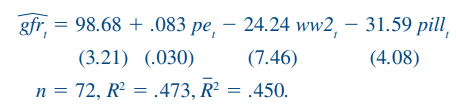
\includegraphics[scale=1.5]{figuras/fertil3.1.png}

\end{centering}

a) (3 puntos) ¿Cuales son los efectos de las variables \textit{ww2} y \textit{pills}? ¿son estadisticamente significativos?

\respuesta El modelo sin tendencia entrega $\widehat\beta_{ww2}=-24{,}24$
($t=-24{,}24/7{,}46\approx-3{,}25$) y $\widehat\beta_{pill}=-31{,}59$
($t=-31{,}59/4{,}08\approx-7{,}74$). Durante la Segunda Guerra Mundial hubo
unos 24 nacimientos menos por cada 1.000 mujeres, y con la píldora unos 32
menos. Ambos efectos son estadísticamente significativos ($|t|>2$).
\fin

Si se añade una tendencia lineal en el tiempo a la ecuación, se obtiene:

\begin{centering}
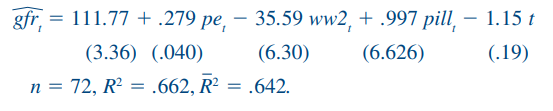
\includegraphics[scale=1.5]{figuras/fertil3.2.png}

\end{centering}

b) (3 puntos) ¿Como interpreta el factor de tendencia?

\respuesta El coeficiente de $t$ es $-1{,}15$ ($t\approx-6{,}05$): manteniendo
constantes las demás variables, la fertilidad cae en promedio 1,15 nacimientos
por cada 1.000 mujeres por año. Es significativo.
\fin

c) (4 puntos) ¿cambian los efectos de \textit{ww2} y \textit{pills}?¿siguen siendo significativos?

\respuesta Sí cambian. \textit{ww2} pasa a $-35{,}59$ ($t\approx-5{,}65$) y
sigue siendo significativo. \textit{pill} pasa a $+0{,}997$ ($t\approx0{,}15$)
y \textbf{deja de ser significativo}. El efecto antes atribuido a la píldora
reflejaba en realidad la tendencia decreciente: el modelo sin tendencia sufría
de variable omitida.
\fin

Ahora añadimos una tendencia cuadratica a la ecuación y obtenemos:

\begin{centering}
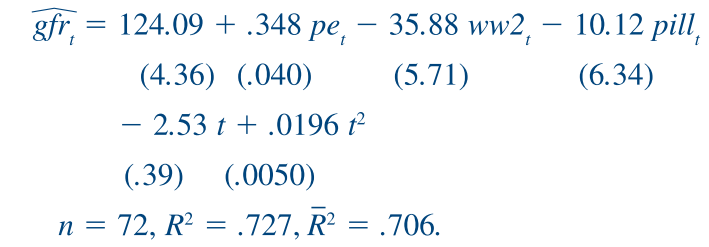
\includegraphics[scale=1]{figuras/fertil3.3.png}

\end{centering}

d) (3 puntos) ¿que logra captar esta tendencia cuadratica?

\respuesta Una tendencia no lineal: con $\widehat\gamma_t=-2{,}53$ y
$\widehat\gamma_{t^2}=0{,}0196$ ($t\approx3{,}9$) la fertilidad cae a un ritmo
decreciente, alcanza un mínimo y luego se recupera (forma de U). El mínimo está en
\[
    t^*=\frac{2{,}53}{2(0{,}0196)}\approx64{,}5,
\]
es decir, hacia 1977. El $\overline R^2$ sube de $0{,}642$ a $0{,}706$ y
\textit{pill} sigue sin ser significativo ($t\approx-1{,}6$).
\fin

e) (3 puntos) ¿será adecuado adicionar una tendencia $t^3$ a nuestro modelo?

\respuesta No necesariamente. Habría que estimarlo y ver si $t^3$ es
significativo (test $t$) y si mejora el $\overline R^2$. Además, $t$, $t^2$ y
$t^3$ están muy correlacionados (colinealidad), hay riesgo de sobreajuste con
solo 72 observaciones y no hay justificación económica para un cambio adicional
de curvatura. La tendencia cuadrática parece suficiente.
\fin

\item\color{black} A partir de la siguiente grafica, responda:

\begin{centering}
    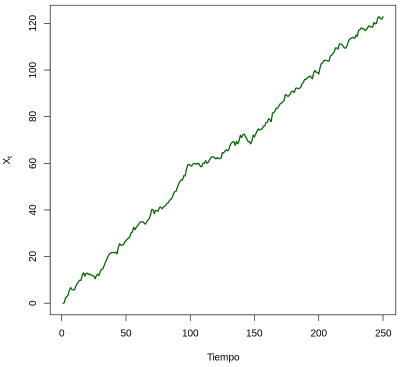
\includegraphics[scale=1]{figuras/Random Walk 1.png}\\
\end{centering}

a) (2 puntos) Según sus conocimientos, a partir de la imagen, usted afirmaria que esta serie es ¿estacionaria o tiene raiz unitaria?

\respuesta La serie presenta una tendencia creciente casi lineal, sin reversión
a una media constante. Visualmente no parece estacionaria: corresponde a una
raíz unitaria con deriva ($X_t=X_{t-1}+0{,}5+\varepsilon_t$).
\fin

b) (3 puntos) Plantee el test Dickey-Fuller

\respuesta Con deriva: $\Delta X_t=\alpha+\gamma X_{t-1}+\varepsilon_t$. Con
tendencia: $\Delta X_t=\alpha+\gamma X_{t-1}+\delta t+\varepsilon_t$. En ambos casos
\[
    H_0:\gamma=0\ \text{(raíz unitaria, no estacionaria)},
    \qquad
    H_1:\gamma<0\ \text{(estacionaria)}.
\]
\fin

c) (5 puntos) Ejecute el test de Dickey-Fuller en R, ¿podemos afirmar o no que la serie de tiempo es estacionaria?

Para plantear el test Dickey-Fuller, utilice el siguiente codigo:

\begin{centering}
    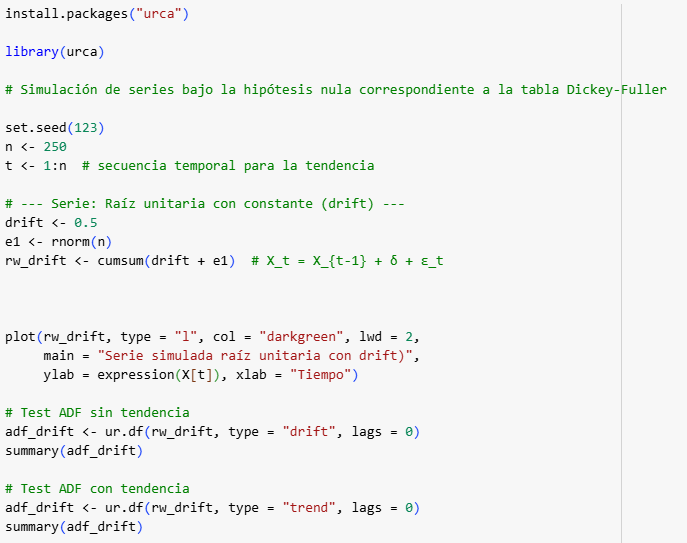
\includegraphics[scale=1]{figuras/Codigo.png}\\
\end{centering}

\respuesta Los resultados de \texttt{ur.df} (salidas \texttt{ADF 1.1} y
\texttt{ADF 1.2}) son:
\begin{center}
\begin{tabular}{lccc}
    \hline
    Modelo & Estadístico $\tau$ & Crítico 5\% & Decisión\\
    \hline
    \texttt{drift} & $-0{,}865$ & $-2{,}88$ & no se rechaza $H_0$\\
    \texttt{trend} & $-3{,}205$ & $-3{,}43$ & no se rechaza $H_0$ (5\%)\\
    \hline
\end{tabular}
\end{center}
(En el modelo \texttt{trend}, al 10\% el crítico es $-3{,}13$ y se rechazaría de
forma marginal; el estadístico conjunto $\phi_3=5{,}35<6{,}49$ tampoco rechaza.)
No hay evidencia suficiente para afirmar que la serie es estacionaria: se
mantiene la hipótesis de raíz unitaria y conviene trabajar en primeras
diferencias. La significancia del término de tendencia ($p=0{,}0018$) no sirve
para inferir, pues bajo raíz unitaria los $t$ usuales no tienen distribución
estándar.
\fin

\item\color{black} Un investigador ha simulado tres series temporales de 200 observaciones. Dos de ellas corresponden a procesos \textbf{AR(1)} con distintos valores del parámetro \( \phi \), y la tercera corresponde a un proceso de \textbf{ruido blanco} (white noise). Para cada caso se presentan dos gráficos:

\begin{itemize}
    \item A la izquierda: la serie temporal simulada \( \{X_t\} \)
    \item A la derecha: su función de autocorrelación (ACF) hasta el rezago 30
\end{itemize}

Los valores de \( \phi \) utilizados para los procesos AR(1) fueron:

\[
\phi = -0.95 \quad \text{y} \quad \phi = 0.95
\]

\[
X_t = \phi X_{t-1} + \varepsilon_t
\]

Los gráficos han sido rotulados como \textbf{Caso A}, \textbf{Caso B} y \textbf{Caso C} (sin indicar el valor de \( \phi \) ni el tipo de proceso que representan).

\begin{enumerate}
    \item (3 puntos) Identifique cuál de los tres casos corresponde al proceso de \textbf{ruido blanco}. Justifique su respuesta con base en el comportamiento de la serie y su ACF.

    \respuesta El \textbf{Caso B} (gráfico central). La serie fluctúa sin patrón
    alrededor de cero y su ACF es prácticamente nula para todos los rezagos
    $k\geq1$, dentro de las bandas de confianza.
    \fin

    \item (5 puntos) Para los otros dos casos, asigne a cada uno el valor de \( \phi \) correspondiente. Justifique su elección explicando cómo el signo y la magnitud de \( \phi \) se reflejan en la dinámica de la serie y en la forma de su ACF.

    \respuesta Para un AR(1), $\rho_k=\phi^k$.
    \begin{itemize}
        \item \textbf{Caso A, $\phi=-0{,}95$}: la serie oscila rápidamente
        alrededor de cero, cambiando de signo casi en cada período. La ACF
        alterna de signo ($\rho_1\approx-0{,}95$, $\rho_2\approx+0{,}90,\dots$) y
        decae lentamente en magnitud.
        \item \textbf{Caso C, $\phi=+0{,}95$}: la serie es suave y persistente,
        con excursiones largas sobre y bajo cero. La ACF es positiva y decae
        lentamente ($\rho_k=0{,}95^k$).
    \end{itemize}
    La magnitud $|\phi|$ cercana a 1 explica el decaimiento lento de la ACF; el
    signo determina si la ACF alterna o no.
    \fin

\end{enumerate}

\begin{figure}[H]
    \centering
    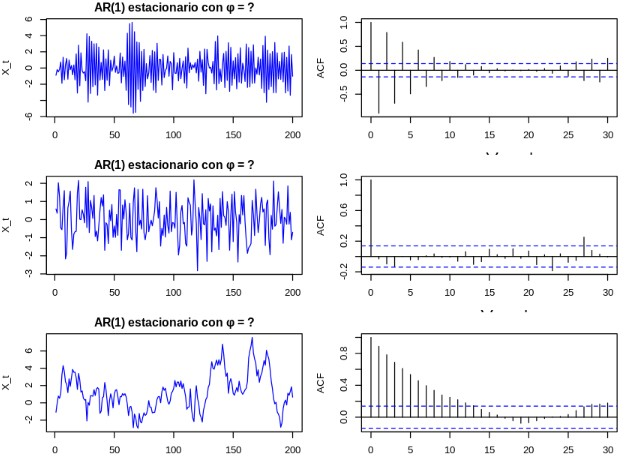
\includegraphics[width=0.7\linewidth]{figuras/autocorr.jpg}
\end{figure}

\item\color{black} A partir de la bases de datos \textit{hprice1} se realiza la siguiente regresión:

\begin{centering}
    $$price = \beta_0 + \beta_1 bdrms + \beta_2 lotsize + \beta_3sqrft$$
\end{centering}

\textit{bdrms:} número de habitaciones
\textit{lotsize:} tamaño del terreno
\textit{sqrtft:} metros cuadrados construidos

a) (2 puntos) Plantee la hipotesis nula del test de Breusch-Pagan

\respuesta Se estima $\widehat u^2=\delta_0+\delta_1bdrms+\delta_2lotsize
+\delta_3sqrft+v$ y se contrasta
\[
    H_0:\delta_1=\delta_2=\delta_3=0
    \quad(\var(u\mid X)=\sigma^2,\ \text{homocedasticidad}),
\]
frente a $H_1$: al menos un $\delta_j\neq0$ (heterocedasticidad).
\fin

b) (4 puntos) Realizamos el test de Breusch-Pagan el cual nos arroja un \textit{p-value = 0.002782} ¿Que consecuencias trae este resultado? ¿Que recomendaría hacer en este caso?

\respuesta Como $p=0{,}0028<0{,}01$, se rechaza $H_0$ incluso al 1\%: hay
heterocedasticidad. MCO sigue siendo insesgado y consistente, pero los errores
estándar usuales son inválidos (también $t$ y $F$) y MCO deja de ser eficiente.
Se recomienda usar errores estándar robustos (White/HC), o bien MCP/MCG
factibles, o estimar el modelo con $\log(price)$, que suele atenuar la
heterocedasticidad.
\fin

\vspace{1.5cm}

\item\color{black} A partir de la base de datos \textit{mlb1} se realiza la siguiente regresión:

\begin{centering}
    $$salary = \beta_0 + \beta_1 teamsal + \beta_2games + \beta_3years + \beta_4atbats$$
\end{centering}

Realizando la regresión en R, nos arrojo los siguientes resultados:

\begin{centering}
    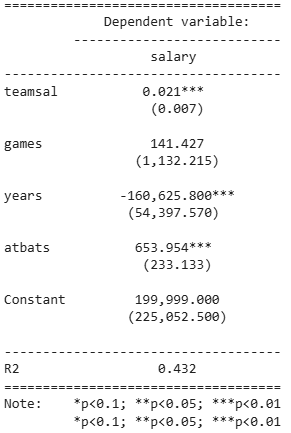
\includegraphics[scale=1]{figuras/mlb1.1.png}\\
\end{centering}

a) (2 puntos) plantee una regresión auxiliar que nos permita encontrar multicolinealidad en la variable \textit{games}

\respuesta
\[
    games=\alpha_0+\alpha_1teamsal+\alpha_2years+\alpha_3atbats+w.
\]
\fin

b) (3 puntos) la regresión auxiliar de \textit{games} nos arrojo $R^2=0.9913$ ¿Cual es el valor del factor de inflación de la varianza? ¿Que se interpreta de este resultado?

\respuesta
\[
    VIF_{games}=\frac{1}{1-0{,}9913}=\frac{1}{0{,}0087}\approx114{,}9,
\]
que coincide con el valor de \texttt{vif} (115,04). La varianza de
$\widehat\beta_{games}$ es unas 115 veces mayor que si \textit{games} no
estuviera correlacionada con los demás regresores, y su error estándar unas
10,7 veces mayor. Esto se ve en la regresión: coeficiente $141{,}4$ con error
estándar $1.132{,}2$, no significativo. Hay multicolinealidad severa.
\fin

c) (5 puntos) Utilizando la función \textit{vif} en R, calculamos el factor de variabilidad de la varianza de cada una de las variables y nos arrojo los siguientes valores para cada una:

\begin{itemize}
    \item games: 115.04
    \item teamsal: 1.03
    \item years: 13.77
    \item atbats: 68.92
\end{itemize}

¿Como podría explicar que las variables \textit{games}, \textit{years} y \textit{atbats} resultarán con VIF sobre 10?
¿Cual sería su recomendación?

\respuesta Las tres variables miden esencialmente la misma dimensión: la
trayectoria del jugador. A más años y más partidos jugados, mecánicamente más
turnos al bate (colinealidad estructural). \textit{teamsal} ($VIF=1{,}03$) no
presenta problema.

La multicolinealidad no sesga los estimadores; solo reduce su precisión. Si el
objetivo es predecir, puede ignorarse. Si se desea interpretar efectos
individuales, conviene eliminar la variable más redundante (\textit{games}, no
significativa) o combinar las variables (por ejemplo, \textit{atbats} por
partido), o contrastar conjuntamente \textit{games} y \textit{atbats} con un
test $F$, que no se ve afectado. No se deben eliminar variables sin respaldo
teórico, pues se introduciría sesgo por variable omitida.
\fin

\item\color{black} A partir de la base de datos \textit{Attend} se construye la siguiente regresión lineal:

\begin{centering}
    $final = \beta_0 + \beta_1attendrte + \beta_2ACT + \beta_3Soph$
\end{centering}

\begin{centering}
    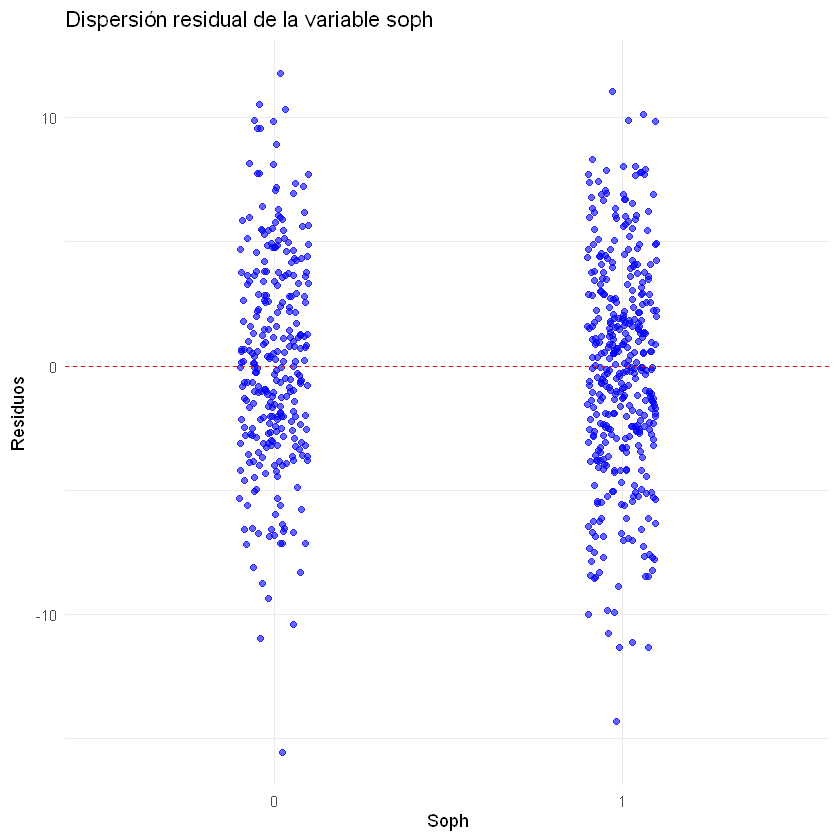
\includegraphics[scale=0.25]{figuras/Shapiro-Wilk.png}\\
\end{centering}

a) (3 puntos) a partir de la imagen, ¿se puede afirmar con certeza que los residuos distribuyen normal? ¿se puede afirmar si hay heterocedasticidad u homocedasticidad?

\respuesta No. Un gráfico de residuos contra una variable binaria solo muestra
la dispersión por grupo, no la forma de la distribución; para evaluar
normalidad se requiere un histograma, un gráfico Q-Q o un test. Respecto de la
varianza, la dispersión es similar en $Soph=0$ y $Soph=1$, lo que sugiere
homocedasticidad respecto de esa variable. Sin embargo, un solo gráfico y un
solo regresor no son concluyentes; se necesita un test formal (Breusch-Pagan o
White).
\fin

b) (3 puntos) Si al realizar el test de Shapiro-Wilk en R nos arroja un \textit{p-value = 0.3619} ¿Que se puede decir de los residuos de la muestra? ¿Que sucederia si \textit{p-value = 0.0001}?

\respuesta El test tiene $H_0$: los residuos son normales.
\begin{itemize}
    \item $p=0{,}3619>0{,}05$: no se rechaza $H_0$; no hay evidencia contra la
    normalidad (lo que no prueba que los residuos sean normales).
    \item $p=0{,}0001<0{,}05$: se rechaza $H_0$; los residuos no son normales.
    Con muestras grandes los estadísticos $t$ y $F$ siguen siendo
    aproximadamente válidos por el teorema central del límite; con muestras
    pequeñas, la inferencia exacta dejaría de ser confiable.
\end{itemize}
\fin

\end{enumerate}

\end{document}
